\documentclass[10pt]{article}

%%%%%%%%%%%%%%%%%%%%%%%%%%%%%%%%%%%%%%%%%%%%%%%%%%%%%%%%%%%%%%%%%%%%%%%%%%%%%%%%
% LaTeX Imports
%%%%%%%%%%%%%%%%%%%%%%%%%%%%%%%%%%%%%%%%%%%%%%%%%%%%%%%%%%%%%%%%%%%%%%%%%%%%%%%%
\usepackage{amsfonts}                                                   % Math fonts
\usepackage{amsmath}                                                    % Math formatting
\usepackage{amssymb}                                                    % Math formatting
\usepackage{amsthm}                                                     % Math Theorems
\usepackage{arydshln}                                                   % Dashed hlines
\usepackage{attachfile}                                                 % AttachFiles
\usepackage{cancel}                                                     % Cancelled math
\usepackage{caption}                                                    % Figure captioning
\usepackage{color}                                                      % Nice Colors
\input{./lib/dragon.inp}                                                % Tikz dragon curve
\usepackage[ampersand]{easylist}                                        % Easy lists
\usepackage{fancyhdr}                                                   % Fancy Header
\usepackage[T1]{fontenc}                                                % Specific font-encoding
%\usepackage[margin=1in, marginparwidth=2cm, marginparsep=2cm]{geometry} % Margins
\usepackage{graphicx}                                                   % Include images
\usepackage{hyperref}                                                   % Referencing
\usepackage[none]{hyphenat}                                             % Don't allow hyphenation
\usepackage{lipsum}                                                     % Lorem Ipsum Dummy Text
\usepackage{listings}                                                   % Code display
\usepackage{marginnote}                                                 % Notes in the margin
\usepackage{microtype}                                                  % Niceness
\usepackage{lib/minted}                                                 % Code display
\usepackage{multirow}                                                   % Multirow tables
\usepackage{pdfpages}                                                   % Include pdfs
\usepackage{pgfplots}                                                   % Create Pictures
\usepackage{rotating}                                                   % Figure rotation
\usepackage{setspace}                                                   % Allow double spacing
\usepackage{subcaption}                                                 % Figure captioning
\usepackage{tikz}                                                       % Create Pictures
\usepackage{tocloft}                                                    % List of Equations
%%%%%%%%%%%%%%%%%%%%%%%%%%%%%%%%%%%%%%%%%%%%%%%%%%%%%%%%%%%%%%%%%%%%%%%%%%%%%%%%
% Package Setup
%%%%%%%%%%%%%%%%%%%%%%%%%%%%%%%%%%%%%%%%%%%%%%%%%%%%%%%%%%%%%%%%%%%%%%%%%%%%%%%%
\hypersetup{%                                                           % Setup linking
    colorlinks=true,
    linkcolor=black,
    citecolor=black,
    filecolor=black,
    urlcolor=black,
}
\RequirePackage[l2tabu, orthodox]{nag}                                  % Nag about bad syntax
\renewcommand*\thesection{\arabic{section} }                             % Reset numbering
\renewcommand{\theFancyVerbLine}{ {\arabic{FancyVerbLine} } }              % Needed for code display
\renewcommand{\footrulewidth}{0.4pt}                                    % Footer hline
\setcounter{secnumdepth}{3}                                             % Include subsubsections in numbering
\setcounter{tocdepth}{3}                                                % Include subsubsections in toc
%%%%%%%%%%%%%%%%%%%%%%%%%%%%%%%%%%%%%%%%%%%%%%%%%%%%%%%%%%%%%%%%%%%%%%%%%%%%%%%%
% Custom commands
%%%%%%%%%%%%%%%%%%%%%%%%%%%%%%%%%%%%%%%%%%%%%%%%%%%%%%%%%%%%%%%%%%%%%%%%%%%%%%%%
\newcommand{\nvec}[1]{\left\langle #1 \right\rangle}                    %  Easy to use vector
\newcommand{\ma}[0]{\mathbf{A} }                                         %  Easy to use vector
\newcommand{\mb}[0]{\mathbf{B} }                                         %  Easy to use vector
\newcommand{\abs}[1]{\left\lvert #1 \right\rvert}                       %  Easy to use abs
\newcommand{\pren}[1]{\left( #1 \right)}                                %  Big parens
\let\oldvec\vec
\renewcommand{\vec}[1]{\oldvec{\mathbf{#1} } }                            %  Vector Styling
\newtheorem{thm}{Theorem}                                               %  Define the theorem name
\newtheorem{definition}{Definition}                                     %  Define the definition name
\definecolor{bg}{rgb}{0.95,0.95,0.95}
\newcommand{\java}[4]{\vspace{10pt}\inputminted[firstline=#2,
                                 lastline=#3,
                                 firstnumber=#2,
                                 gobble=#4,
                                 frame=single,
                                 label=#1,
                                 bgcolor=bg,
                                 linenos]{java}{#1} }
\newcommand{\python}[4]{\vspace{10pt}\inputminted[firstline=#2,
                                 lastline=#3,
                                 firstnumber=#2,
                                 gobble=#4,
                                 frame=single,
                                 label=#1,
                                 bgcolor=bg,
                                 linenos]{python}{#1} }
\newcommand{\js}[4]{\vspace{10pt}\inputminted[firstline=#2,
                                 lastline=#3,
                                 firstnumber=#2,
                                 gobble=#4,
                                 frame=single,
                                 label=#1,
                                 bgcolor=bg,
                                 linenos]{js}{#1} }
%%%%%%%%%%%%%%%%%%%%%%%%%%%%%%%%%%%%%%%%%%%%%%%%%%%%%%%%%%%%%%%%%%%%%%%%%%%%%%%%
% Beginning of document items - headers, title, toc, etc...
%%%%%%%%%%%%%%%%%%%%%%%%%%%%%%%%%%%%%%%%%%%%%%%%%%%%%%%%%%%%%%%%%%%%%%%%%%%%%%%%
\pagestyle{fancy}                                                       %  Establishes that the headers will be defined
\fancyhead[LE,LO]{Computer Systems Notes}                                  %  Adds header to left
\fancyhead[RE,RO]{Zoe Farmer}                                       %  Adds header to right
\cfoot{ \thepage }
\lfoot{CSCI 2400}
\rfoot{Han}
\title{Computer Systems Notes}
\author{Zoe Farmer}

%%%%%%%%%%%%%%%%%%%%%%%%%%%%%%%%%%%%%%%%%%%%%%%%%%%%%%%%%%%%%%%%%%%%%%%%%%%%%%%%
% Beginning of document items - headers, title, toc, etc...
%%%%%%%%%%%%%%%%%%%%%%%%%%%%%%%%%%%%%%%%%%%%%%%%%%%%%%%%%%%%%%%%%%%%%%%%%%%%%%%%
\pagestyle{fancy}                                                       %  Establishes that the headers will be defined
\fancyhead[LE,LO]{Problem Set 2}                                  %  Adds header to left
\fancyhead[RE,RO]{Zoe Farmer}                                       %  Adds header to right
\cfoot{\mlptikz[size=0.25in, text=on, textposx=0, textposy=0, textvalue=\thepage, textscale=0.75in]{applejack}}
\lfoot{CSCI 3104}
\rfoot{Clauset}
\title{Problem Set Two}
\author{Zoe Farmer}
%%%%%%%%%%%%%%%%%%%%%%%%%%%%%%%%%%%%%%%%%%%%%%%%%%%%%%%%%%%%%%%%%%%%%%%%%%%%%%%%
% Beginning of document items - headers, title, toc, etc...
%%%%%%%%%%%%%%%%%%%%%%%%%%%%%%%%%%%%%%%%%%%%%%%%%%%%%%%%%%%%%%%%%%%%%%%%%%%%%%%%
\begin{document}

\maketitle

\begin{easylist}[enumerate]
    @ Consider the following Python function:

        \begin{pythoncode*}{gobble=12}
            def find(a, target):
                x = 0
                y = len(a)
                while x < y:
                    m = (x + y) / 2
                    if a[m] < target:
                        x = m + 1
                    elif a[m] > target:
                        y = m
                    else:
                        return m
            return -1
        \end{pythoncode*}

      Suppose list a has n elements and is sorted.
    @@ Using $\Theta$ notation, what is the best case running time as function of $n$?
    @@@ $\Theta(1) \to$ If the target is the middle element the algorithm completes in constant time.
    @@ Using $\Theta$ notation, what is the worst case running time as function of $n$?
    @@@ $\Theta(\log_2(n)) \to$ If the target is at one end, the algorithm will divide the array in half each time until the target is found.

    @ In the classic version of Quicksort, the pivot is always chosen as the last element in the input array. When the pivot is compared to another element, we can use any valid comparison operator. Thus, ``sorting'' generalizes to any set of inputs over which we can mathematically define comparisons.

    Use this version of the algorithm to sort the following functions by order of asymptotic growth such that the final arrangement of functions $g_1, g_2, \cdots, g_{12}$ satisfies the ordering constraint $g_1 = \Omega(g_2), g_2 = \Omega(g_3), \cdots, g_{11} = \Omega(g_{12})$.

    \begin{center}
        \begin{tabular}{|l|}
            \hline
            $n$\\
            \hline
            $n^2$\\
            \hline
            ${\left( \sqrt{2} \right)}^{\log_2(n)}$\\
            \hline
            $2^{\log^*_2(n)}$\\
            \hline
            $n!$\\
            \hline
            $(\log_2(n))!$\\
            \hline
            ${ \left( \frac{3}{2} \right) }^n$\\
            \hline
            $n^{\frac{1}{\log_2(n)}}$\\
            \hline
            $n \log_2(n)$\\
            \hline
            $\log_2(n!)$\\
            \hline
            $e^n$\\
            \hline
            $1$\\
            \hline
        \end{tabular}
    \end{center}

    @@ For each branch of the recursion tree, identify the chosen pivot element; for each level of the recursion tree and after all pivot elements at that level have been moved into their final location, give the global array ordering.  (Hint: it may be easier to work out the final ordering by hand and then backtrack through the Quicksort operations to produce the recursion tree.)
    @@@ Solving the ordering first allows us to obtain the array representing the order of the given array:

        \setcounter{MaxMatrixCols}{20}
        \[
        \scalebox{0.75}{$
            \begin{matrix}
                n & n^2 & {\left( \sqrt{2} \right)}^{\log_2(n)} & 2^{\log^*_2(n)} & n! & (\log_2(n))! & { \left( \frac{3}{2} \right) }^n & n^{\frac{1}{\log_2(n)}} & n \log_2(n) & \log_2(n!) & e^n & 1\\
                \hline
                5 & 9 & 3 & 4 & 12 & 8 & 10 & 2 & 7 & 6 & 11 & 1
            \end{matrix}
        $}
        \]

        We can use Quicksort to sort this array. See Figure~\ref{fig:pivots}. Each node is the pivot for that step.

        \begin{figure}[ht]
            \centering
            \scalebox{1}{%
            \begin{tikzpicture}
                \node[circle,draw,label={[label distance=0.1cm]0:$[5, 9, 3, 4, 12, 8, 10, 2, 7, 6, 11, 1]$}](z){$1$}
                child[missing]
                child{%
                  node[circle,draw,label={[label distance=0.1cm]0:$[1, 9, 3, 4, 12, 8, 10, 2, 7, 6, 11, 5]$}]{5}
                    child{%
                      node[circle,draw,label={[label distance=0.1cm]180:$[1, 3, 4, 2]$}](A){2}
                      child{%
                        node[circle,draw,label={[label distance=0.1cm]180:$[1]$}](D){1}
                        child[missing]
                        child[missing]
                      }
                      child{%
                        node[circle,draw,label={[label distance=0.1cm]0:$[4, 3]$}](B)[right=1cm of D]{3}
                        child[missing]
                        child{%
                          node[circle,draw,label={[label distance=0.1cm]180:$[4]$}](C){4}
                          child[missing]
                          child[missing]
                        }
                      }
                    }
                    child{%
                      node[circle,draw,label={[label distance=0.1cm]0:$[8, 10, 9, 7, 6, 11, 12]$}][right=4cm of A]{12}
                      child{%
                        node[circle,draw,label={[label distance=0.1cm]0:$[8, 10, 9, 7, 6, 11]$}]{11}
                        child{%
                          node[circle,draw,label={[label distance=0.1cm]0:$[8, 10, 9, 7, 6]$}]{6}
                          child{%
                            node[circle,draw,label={[label distance=0.1cm]0:$[10, 9, 7, 8]$}]{8}
                            child{%
                              node[circle,draw,label={[label distance=0.1cm]180:$[7]$}]{7}
                              child[missing]
                              child[missing]
                            }
                            child{%
                              node[circle,draw,label={[label distance=0.1cm]0:$[10, 9]$}]{9}
                              child{%
                                node[circle,draw,label={[label distance=0.1cm]0:$[10]$}]{10}
                                child[missing]
                                child[missing]
                              }
                              child[missing]
                            }
                          }
                          child[missing]
                        }
                        child[missing]
                      }
                      child[missing]
                    }
                };
            \end{tikzpicture}
        }
            \caption{Quicksort Binary Tree with Pivots}
            \label{fig:pivots}
        \end{figure}

        At each step the array is in a certain order, as is displayed in Table~\ref{table:order}.

        \begin{table}[ht]
            \centering
            \begin{tabular}{| l | l |}
                \hline
                1 & [5, 9, 3, 4, 12, 8, 10, 2, 7, 6, 11, 1]\\
                2 & [1, 9, 3, 4, 12, 8, 10, 2, 7, 6, 11, 5]\\
                3 & [1, 3, 4, 2, 5, 8, 10, 9, 7, 6, 11, 12]\\
                4 & [1, 2, 4, 3, 5, 8, 10, 9, 7, 6, 11, 12]\\
                5 & [1, 2, 3, 4, 5, 6, 8, 10, 9, 7, 11, 12]\\
                6 & [1, 2, 3, 4, 5, 6, 10, 9, 7, 8, 11, 12]\\
                7 & [1, 2, 3, 4, 5, 6, 7, 8, 10, 9, 11, 12]\\
                8 & [1, 2, 3, 4, 5, 6, 7, 8, 9, 10, 11, 12]\\
                \hline
            \end{tabular}
            \caption{Global Array at Each Step}
            \label{table:order}
        \end{table}

    \newpage
    @@ Give the final sorted list and identify which pair(s) functions $f(n)$, $g(n)$, if any, are in the same equivalence class, i.e., $f(n) = \Theta(g(n))$.
    @@@ The resulting array is shown below.

    \begin{center}
        \begin{tabular}{|l|l|}
            \hline
            1 & $1$\\
            \hline
            2 & $n^{\frac{1}{\log_2(n)}}$\\
            \hline
            3 & ${\left( \sqrt{2} \right)}^{\log_2(n)}$\\
            \hline
            4 & $2^{\log^*_2(n)}$\\
            \hline
            5 & $n$\\
            \hline
            6 & $\log_2(n!)$\\
            \hline
            7 & $n \log_2(n)$\\
            \hline
            8 & $(\log_2(n))!$\\
            \hline
            9 & $n^2$\\
            \hline
            10 & ${ \left( \frac{3}{2} \right) }^n$\\
            \hline
            11 & $e^n$\\
            \hline
            12 & $n!$\\
            \hline
        \end{tabular}
    \end{center}

    @ Consider the following recursive function {\ttfamily f}, which takes an integer argument {\ttfamily n} and returns some other integer {\ttfamily f(n)}:

        \begin{pythoncode*}{gobble=12}
            def f(n)
                if n == 0
                    return 3;
                else if n == 1
                    return 5;
                else
                    val = 3 * f(n-1);
                    val = val - 2 * f(n-2);
                    return val;
        \end{pythoncode*}

    @@ Write down the recurrence relation for the value returned by {\ttfamily f(n)}; identify the base cases.
    @@@
        \[ \begin{cases}
                T(n) = 3 \cdot T(n - 1) - 2 \cdot T(n - 2)\\
                T(0) = 3\\
                T(1) = 5
            \end{cases} \]
    @@ Using the method of the characteristic polynomial, solve the value recurrence relation exactly. (See \url{http://bit.ly/1dcsNUJ})

    \[
        \begin{aligned}
            \text{Given: }                         & \to & T(n) = 3 \cdot T(n - 1) - 2 \cdot T(n - 2)\\
            \text{Assume }                         & \to & a_n = c r^n\\
            \text{We can represent $T(n)$ as }     & \to & a_n = 3 a_{n-1} - 2 a_{n-2}\\
            \text{Substituting }                   & \to & c r^n = 3cr^{n-1} - 2 c r^{n-2}\\
            \text{Characteristic Polynomial Roots} & \to & -r^2 + 3r -2 = 0 \to \text{Roots: } [1, 2]\\
            \text{Therefore}                       & \to & a_n = c_1 + c_2 2^n\\
            \text{Using our base cases: }          & \to & \begin{cases} 3 = c_1 + c_2\\5 = c_1 + 2 c_2 \end{cases}\\
            \text{Therefore}                       & \to & c_1 = 1, c_2 = 2\\
            \text{Therefore}                       & \to & \boxed{a_n = 2^{n+1} + 1}_\blacksquare
        \end{aligned}
    \]

    @@ Show (prove) by induction that your solution is correct.
    @@@ Let $P(n)$ be our propositional function:

        \[ \begin{cases}
            P(n) \equiv 3 a_{n-1} - 2 a_{n-2} = 2^{n+1} + 1\\
            P(0) \equiv 3\\
            P(1) \equiv 5
        \end{cases} \]

    @@@ Show $P(2)$

        \[ 3 \cdot 5 - 2 \cdot 3 = 2^{3} + 1 \Rightarrow 9 = 9 \]

    @@@ Assume $P(k)$. Also assume that $P(k) \Rightarrow P(k + 1)$

        \[ \begin{aligned}
                3 a_{k-1} - 2 a_{k-2} = 2^{k+1} + 1 \Rightarrow 3 a_{k} - 2 a_{k-1} = 2^{k+2} + 1\\
                a_{k-1} = 2^k + 1\\
                3 \cdot 2^{k + 1} + 3 - 2 \cdot 2^k - 2 = 2^{k+2} + 1\\
                3 \cdot 2^{k+1} - 2 \cdot 2^k = 2^{k+2}\\
                3 \cdot 2^{k+1} - 2^{k+1} = 2^{k+2}\\
                {2^{k+2} = 2^{k+2}}_\blacksquare\\
            \end{aligned} \]

    @@ Under the {\ttfamily RAM} model of computation, write down the recurrence relation for the running time of {\ttfamily f(n)}.
    @@@ The recurrence relation above can be redefined in terms of operations.

        \[ T(n) = \overbrace{\underbrace{3 \cdot T}_1 (\overbrace{n-1}^1) - \underbrace{2 \cdot T}_1 (\overbrace{n-2}^1)}^{1} \]

        As you can see, each level requires 5 operations and is called twice. This allows us to define the the running time of the recurrence relation as

        \[ R(n) = 2 \cdot R(n - 1) + 5 \]

        This overcounts the total number of operations by one, and so our base case is $R(1) = 5$

    @@ Give a succinct explanation in terms of the shape of the recursion tree of why $O(2^n)$ is a trivial upper bound on the running time.
    @@@ At any given node of the binary tree there will either be two children or none, which would indicate that the branch bottomed out at a base case. This means that there are $n$ levels of the tree, and at each level there are $2^n$ branches.
    @@ Using the method of characteristic polynomials, solve the time recurrence relation for a tight upper bound. (Hint: $O(2^n)$ is not tight.)
    \[
        \begin{aligned}
            \text{Given: }                         & \to & R(n) = 2 \cdot R(n - 1) + 5\\
            \text{Assume }                         & \to & a_n = c r^n\\
            \text{We can represent $R(n)$ as }     & \to & a_n = 2 a_{n-1} + 5\\
            \text{Substituting }                   & \to & c r^n = 3cr^{n-1} + 5\\
            \text{Characteristic Polynomial Roots} & \to & -r^2 + 2r = 0 \to \text{Roots: } [0, 2]\\
            \text{Therefore}                       & \to & a_n = c_2 2^n - 1\\
            \text{Using our base case: }           & \to & 5 = c_2\\
            \text{Therefore}                       & \to & \boxed{5(2^n - 1)}_\blacksquare
        \end{aligned}
    \]

    \newpage
    @ Solve the following recurrence relations using the method specified. Show your work.
    @@ $T(n) = T (n − 1) + n$ by unrolling (tail recursion).
    @@@ Tail Recursion involved substituting the next step into the current one, and then estimating an answer based on the results.

        \[
            \begin{matrix}
                T(n) = T(n - 1) + n      & \to & T(n - 1) = T(n - 2) + n - 1\\
                T(n) = T(n - 2) + 2n - 1 & \to & T(n - 2) = T(n - 3) + n - 2\\
                T(n) = T(n - 3) + 3n - 3 & \to & T(n - 3) = T(n - 4) + n - 3\\
                T(n) = T(n - 4) + 4n - 6 & & \\
                \boxed{T(n) = c + \frac{1}{2} n ( n + 1)}_\blacksquare
            \end{matrix}
        \]

    @@ $T(n) = 2T \left( \frac{n}{2} \right) + n^3$ by the Master method.
    @@@ The Master Method states that for a recurrence relation of the form
        \[ T(n) = a T\left( \frac{n}{b} \right) + f(n) \]
        if $f(n) = \Theta(n^c)$ where $c > \log_b(a)$, then $T(n) = \Theta(f(n))$. In this problem, $3 > \log_2(2)$, therefore 
        \[ \boxed{T(n) = \Theta(n^3)} \]

    \newpage
    @ Professor Septima Vector thinks she has discovered a remarkable property of binary search trees. Suppose that the search for key $k$ in a binary search tree ends up in a leaf. Consider three (possibly empty) sets: $A$, the keys to the left of the search path; $B$, the keys on the search path; and $C$, the keys to the right of the search path.  Professor Vector claims that any three keys $a \in A$, $b \in B$ and $c \in C$ must satisfy $ a \le b \le c$. Prove that Vector's claim is false by giving a counterexample that is the smallest possible.
    @@ The easiest counterexample given the phrasing of her property is when $k$ is the smallest element in the tree. In this case, $A = \emptyset$ and thusly no key $a$ could possibly be in $A$, $\not\exists a$. However, depending on the meaning of the question it could also be interpreted that this case falls to $b \le c$ which is true.

    Therefore an alternate counterexample is when there is a zig-zag in the nodes. Please reference Figure~\ref{fig:counter} for a pictoral representation. If $k = 7$, then $A = {3, 6}, B = {10, 5, 7},$ and $C = {15}$. If $ a = 6, b = 5,$ and $c=15$ then Professor Vector's property states that $ 6 \le 5 \le 15$ which is clearly false.

    \begin{figure}[ht]
        \centering
        \scalebox{1}{%
        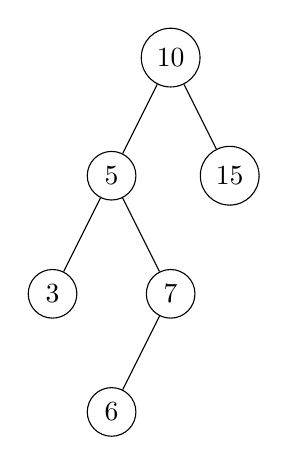
\begin{tikzpicture}
        \node[circle,draw](z){$10$}
            child{%
                node[circle,draw]{5}
                  child{%
                    node[circle,draw]{3}
                    child[missing]
                    child[missing]
                  }
                  child{%
                    node[circle,draw]{7}
                    child{%
                      node[circle,draw]{6}
                      child[missing]
                      child[missing]
                    }
                    child[missing]
                  }
                }
            child{%
                node[circle,draw]{15}
                  child[missing]
                  child[missing]
                };
        \end{tikzpicture}
    }
        \caption{Counterexample Binary Tree}
        \label{fig:counter}
    \end{figure}
\end{easylist}

\end{document}
